\subsection{Distribution - Middleware layer}
This section presents the services that make the middleware up.

Before seeing every service in detail, it is useful to have an overview to the
organization of those components.

\begin{figure}[H]
  \centering
  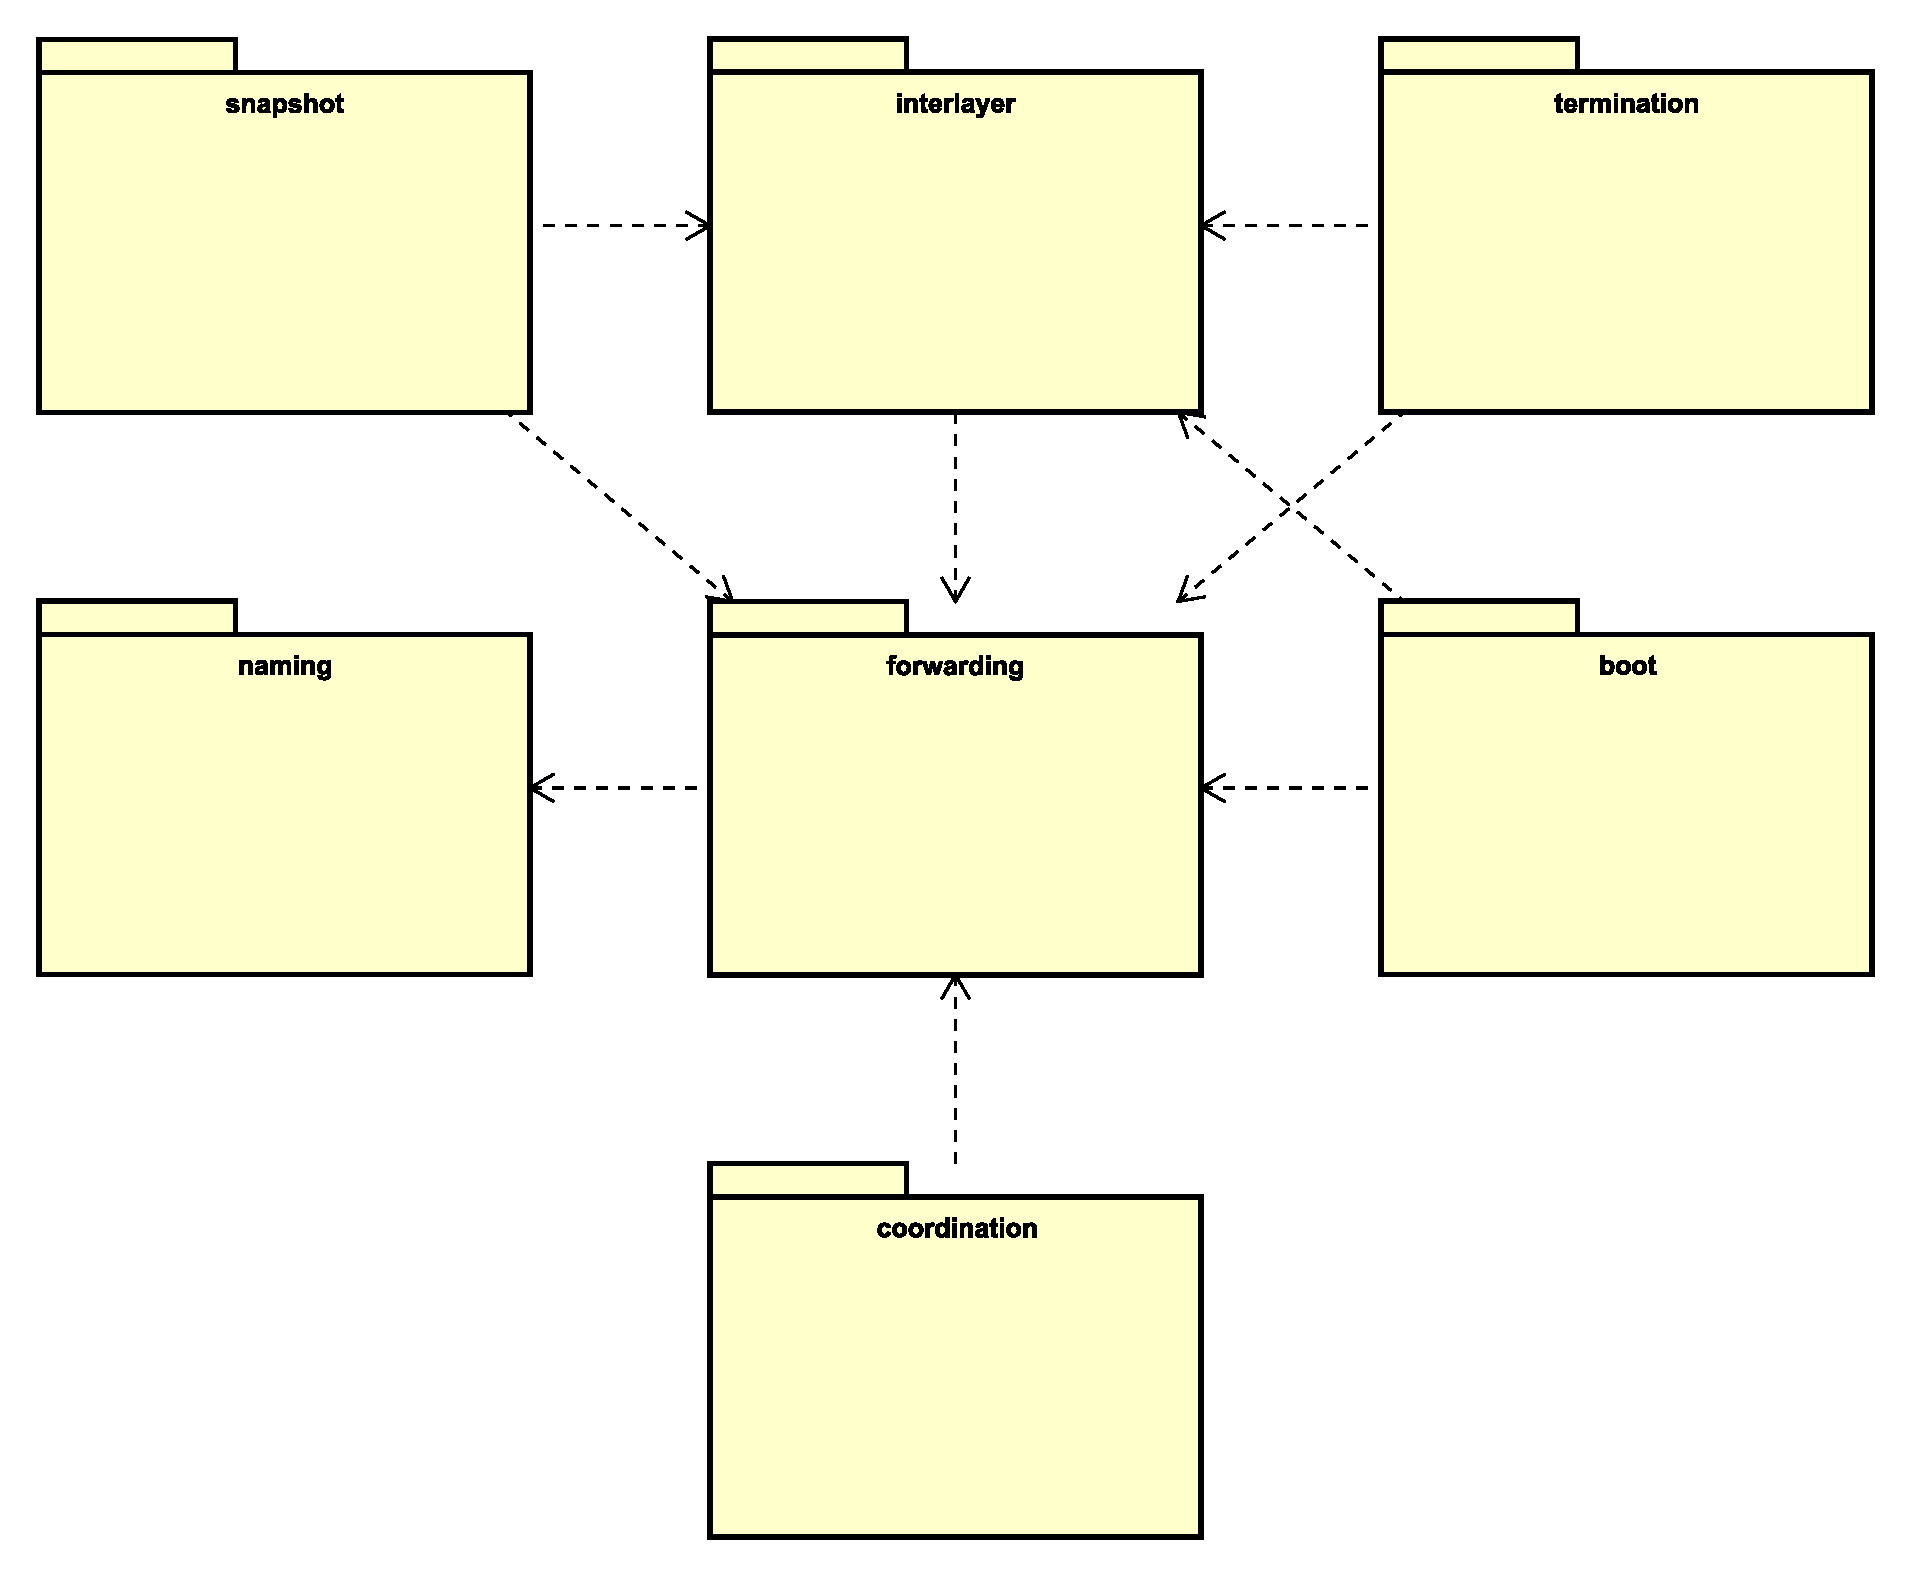
\includegraphics[width=\columnwidth]{images/solution/mw/overview.eps}
  \caption{Middleware architecture overview}
  \label{fig:mw-arch-over}
\end{figure} % TODO: Remove naming package

\begin{itemize}
  \item \texttt{naming}: service that provides a correspondence between logic
    names and actual network addresses;
  \item \texttt{forwarding}: service that represents the abstraction through
    which it is possible to deliver messages to other middleware nodes;
  \item \texttt{interlayer}: service that represents the interface between
    the application and middleware layers;
  \item \texttt{boot}: service that is responsible to start the system neatly;
  \item \texttt{termination}: service that shut downs the node and the system
    neatly;
  \item \texttt{snapshot}: service that takes consistent views of the node and
    the system;
  \item \texttt{coordination}: service that coordinates the interaction among
    the nodes of the system.
\end{itemize}

We thought that it would have been a good situation for using the Fa\c cade
pattern, so each one of the services in figure \ref{fig:mw-arch-over} will have
a ``Fa\c cade module'', that is the interface through which requests are made
to a specific component.
These modules will be recognizable since they will have the same name as the
component they are contained in.

\subsubsection{Naming service}
The Naming service, provided with an entity id and its type, finds the node on
which a given entity resides.

This is done in a completely decoupled way with respect to the application
layer, which just provides the identifier and the type of the entity in the
headers of the message handed over to the middleware. Then, the middleware
Naming component will just have to look for this entity in a configuration
file.

\subsubsection{Forwarding service}
The Forwarding service has to deliver messages to other nodes. This component
is very simple, since it just has an interface (\texttt{MQProxy}) and its
implementation, \texttt{RabbitSender}.

Basically, a \texttt{RabbitSender} takes a message as input and guarantees to
send it to the intended recipient, which could be middleware node or a
RabbitMQ pub/sub queue directed to our brokers.
\texttt{RabbitSender}s are able to make this decision by simply looking if the
messages they are handling are events or node-to-node communication. In the
first case (events), messages are propagated towards the frontend of the
application (and therefore to the brokers). In the other case, messages are
just sent to the node the sender finds in the recipient field of the message.

\subsubsection{Interlayer service}

This component is responsible of the communication that is performed among
different layers, namely the one which it belongs (the \textbf{middleware}) and
another one who uses the middleware layer, that is the \textbf{application}
layer.

We show in figure \ref{fig:mw-interlayer} the architecture of this service and
then we will show in detail each module that composes this component.

\begin{figure}[H]
  \centering
  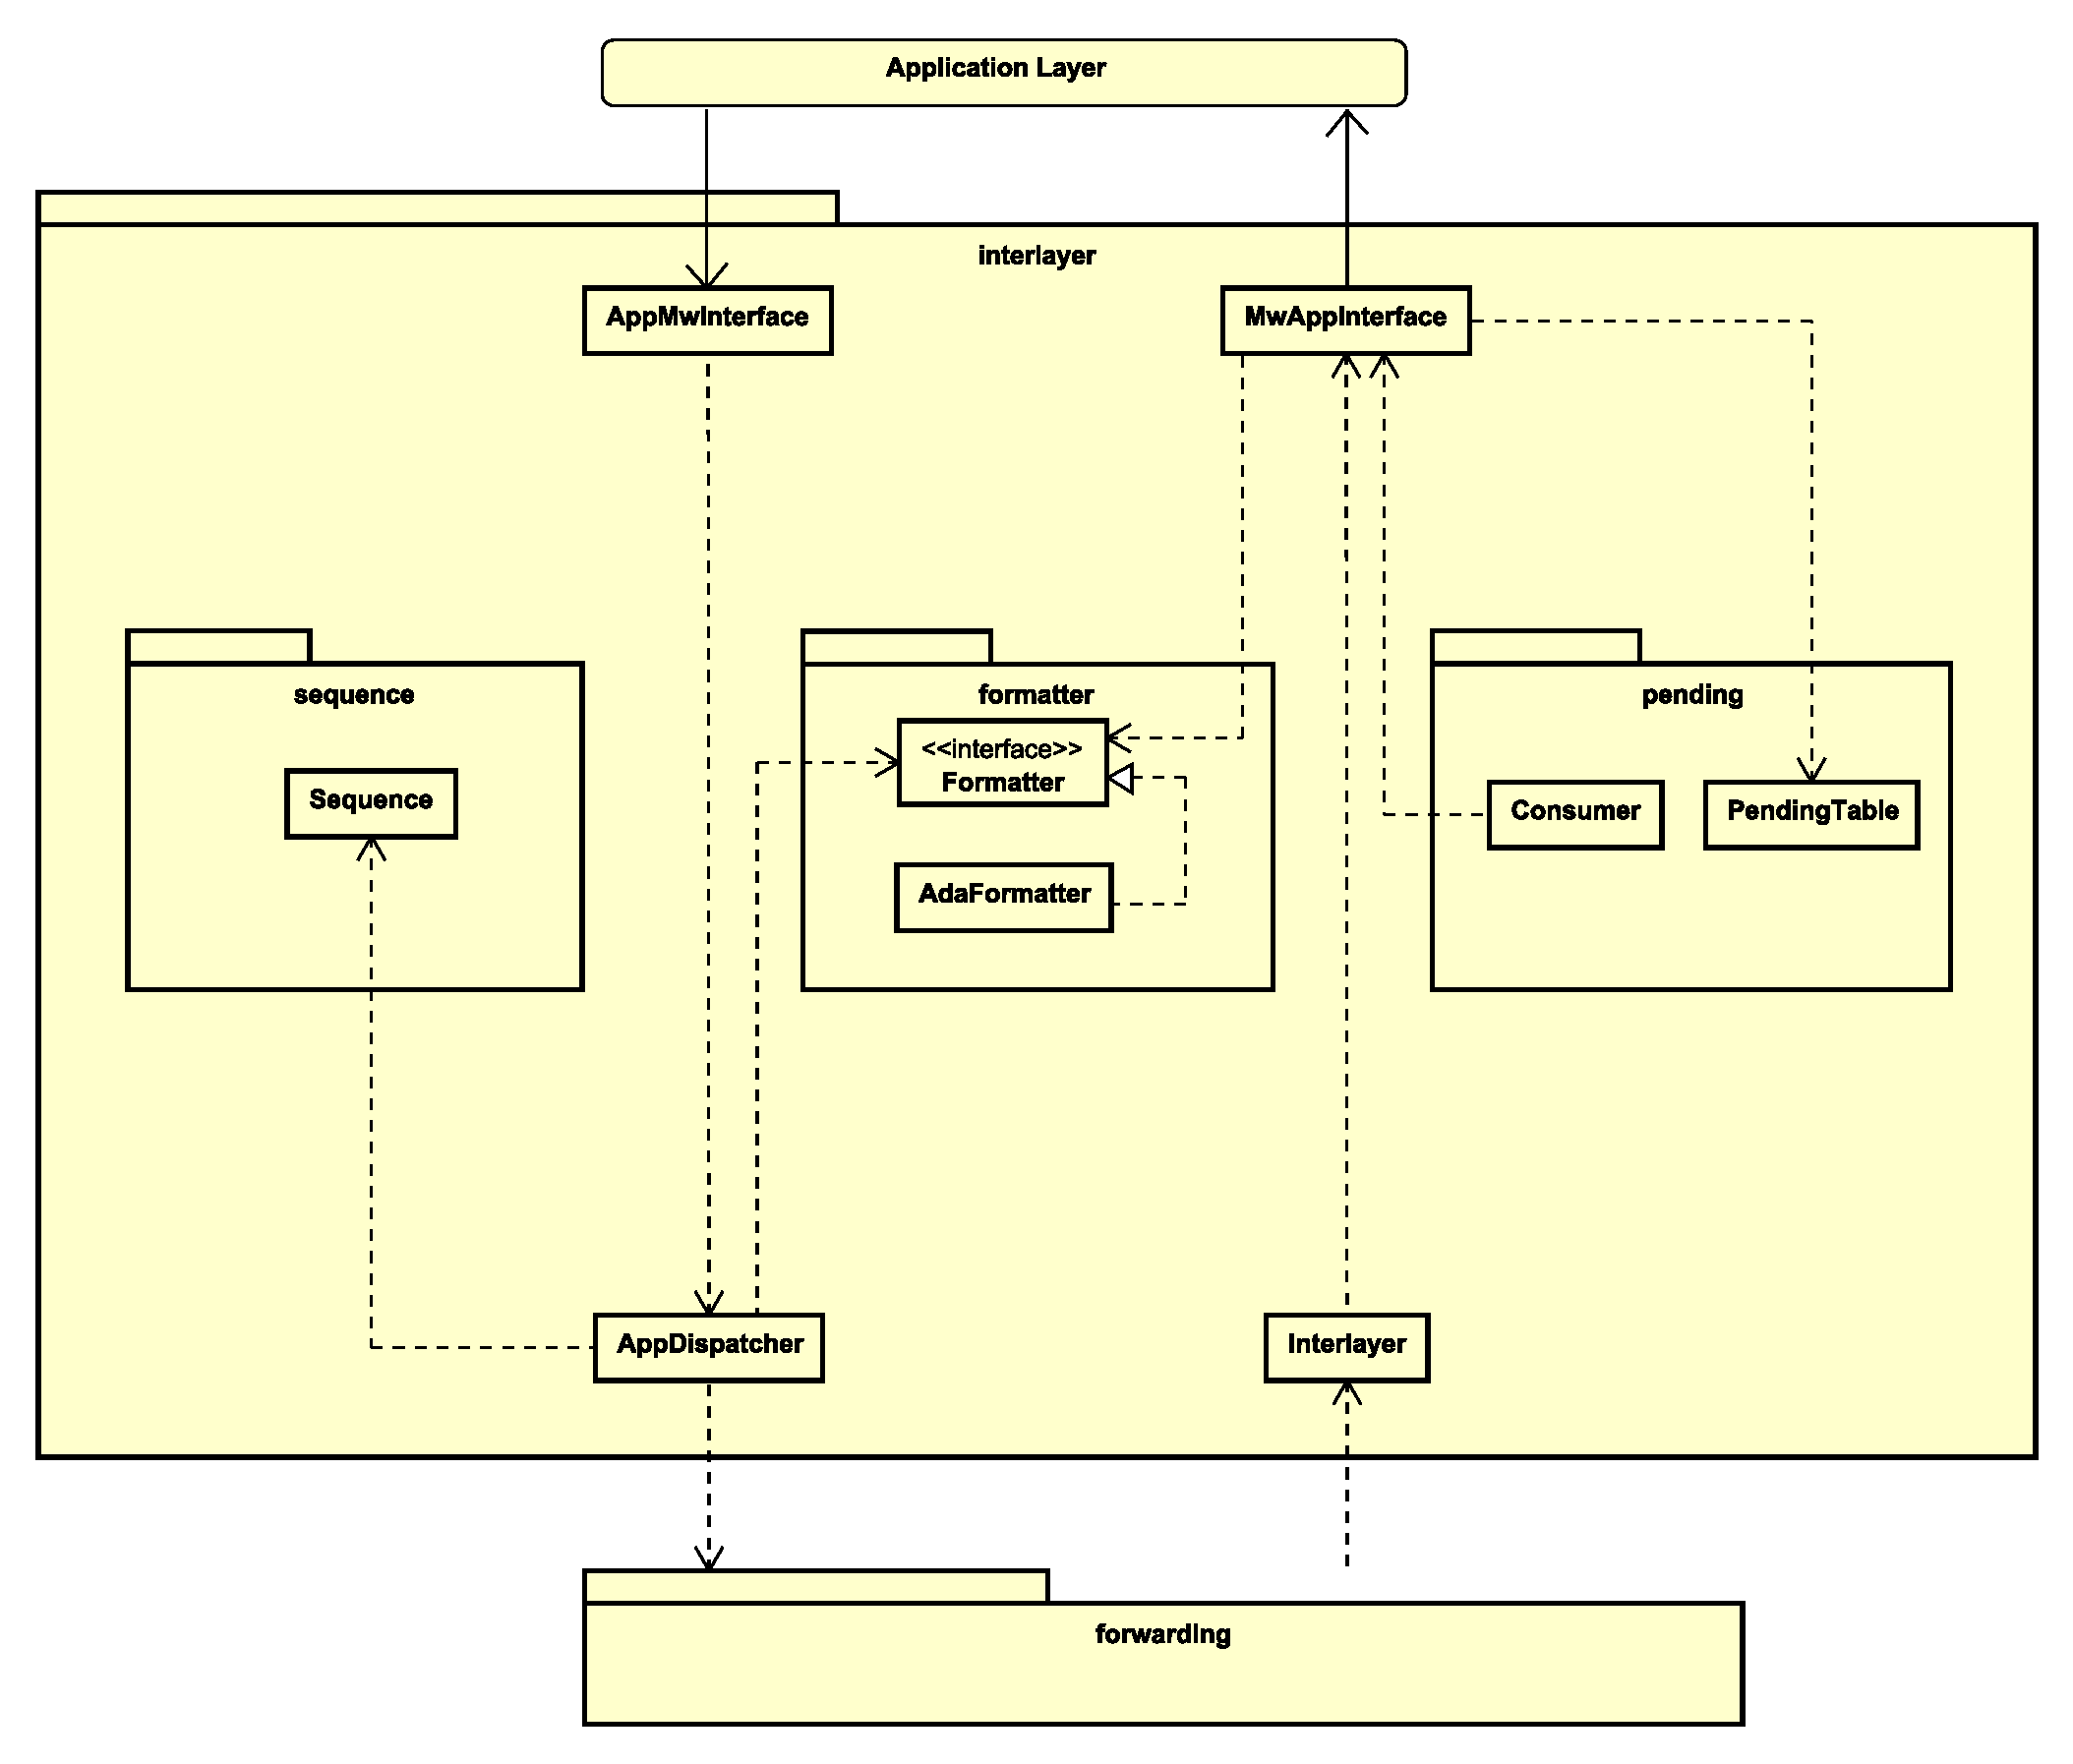
\includegraphics[width=\columnwidth]{images/solution/mw/interlayer.eps}
  \caption{Middleware's Interlayer service}
  \label{fig:mw-interlayer}
\end{figure} % TODO: needs update (Sequence usage comes from AppMwInterface)

% TODO: All class diagrams has to be added
\subsubsubsection{interlayer.Interlayer}

\subsubsubsection{interlayer.MwAppInterface}

\subsubsubsection{interlayer.AppMwInterface}

\subsubsubsection{interlayer.AppDispatcher}

\subsubsubsection{interlayer.sequence.Sequence}

\subsubsubsection{interlayer.formatter.Formatter}

\subsubsubsection{interlayer.formatter.AdaFormatter}

\subsubsubsection{interlayer.pending.PendingTable}

\subsubsubsection{interlayer.pending.Consumer}

\subsubsection{Boot service}\label{sec:mw-boot-descr}

The Boot service is responsible of starting the system in a graceful fashion.
It does so by dividing the start phase into two subphases, namely the
\textbf{marker diffusion} and the \textbf{(own) boot} phase. The procedure is
the same shown in Figure \ref{fig:sys-bootstrap-protocol}, with the first phase
going from left to right and the second phase going in the opposite direction.

In this context, by \textit{marker} we will mean \textit{boot marker}.

When receiving a marker, this the Boot service will forward the marker to all
of its adjacent middleware nodes.
Then, when receiving further markers, this service will just reply immediately
with an end marker.

After having received all the replies for the markers, the Boot service will
request to the application layer to gracefully start.
When the application layer will inform the middleware it started, this service
will send an end marker to all of its adjacent middleware nodes.

\subsubsection{Termination service}

The Termination service is responsible of shutting down the system gracefully.
It does in a symmetrical way to what we have seen in Section
\ref{sec:mw-boot-descr} for the Boot service.

Initially, this service is in a \texttt{running} state, which means the
application layer is normally running.

If the middleware receives a stop marker, it will forward the request marker to
all of its neighbors and any of the subsequent incoming request markers will
receive an immediate reply to fulfill the request.

Then, when the Termination service receives all the replies for the stop marker
from its neighbors, it will send a reply back for the stop request marker and
enter a \texttt{terminating} state, sending an asynchronous request to the
application to stop.

During this second phase, the middleware will wait for a termination marker.
When it arrives, it will forward the termination request marker to all of its
neighbors and reply immediately to any other termination request marker which
arrives by fulfilling it.

As soon as the application will inform the middleware layer that the former is
stopped, the latter will enter a \texttt{stopped} state.

The Termination service will wait both for all of the neighbors to send back a
reply to the termination marker and for itself to enter the \texttt{stopped}
state.
After this, the node will send back a reply for the termination request, ending
the termination procedure for the current node and entering the
\texttt{terminated} state.

%TODO: Add picture

\subsubsection{Snapshot service}
This component is responsible of taking snapshots.

We show in figure \ref{fig:mw-snapshot} the architecture of this service and
then we will show in detail each module that composes this component.

\begin{figure}[H]
  \centering
  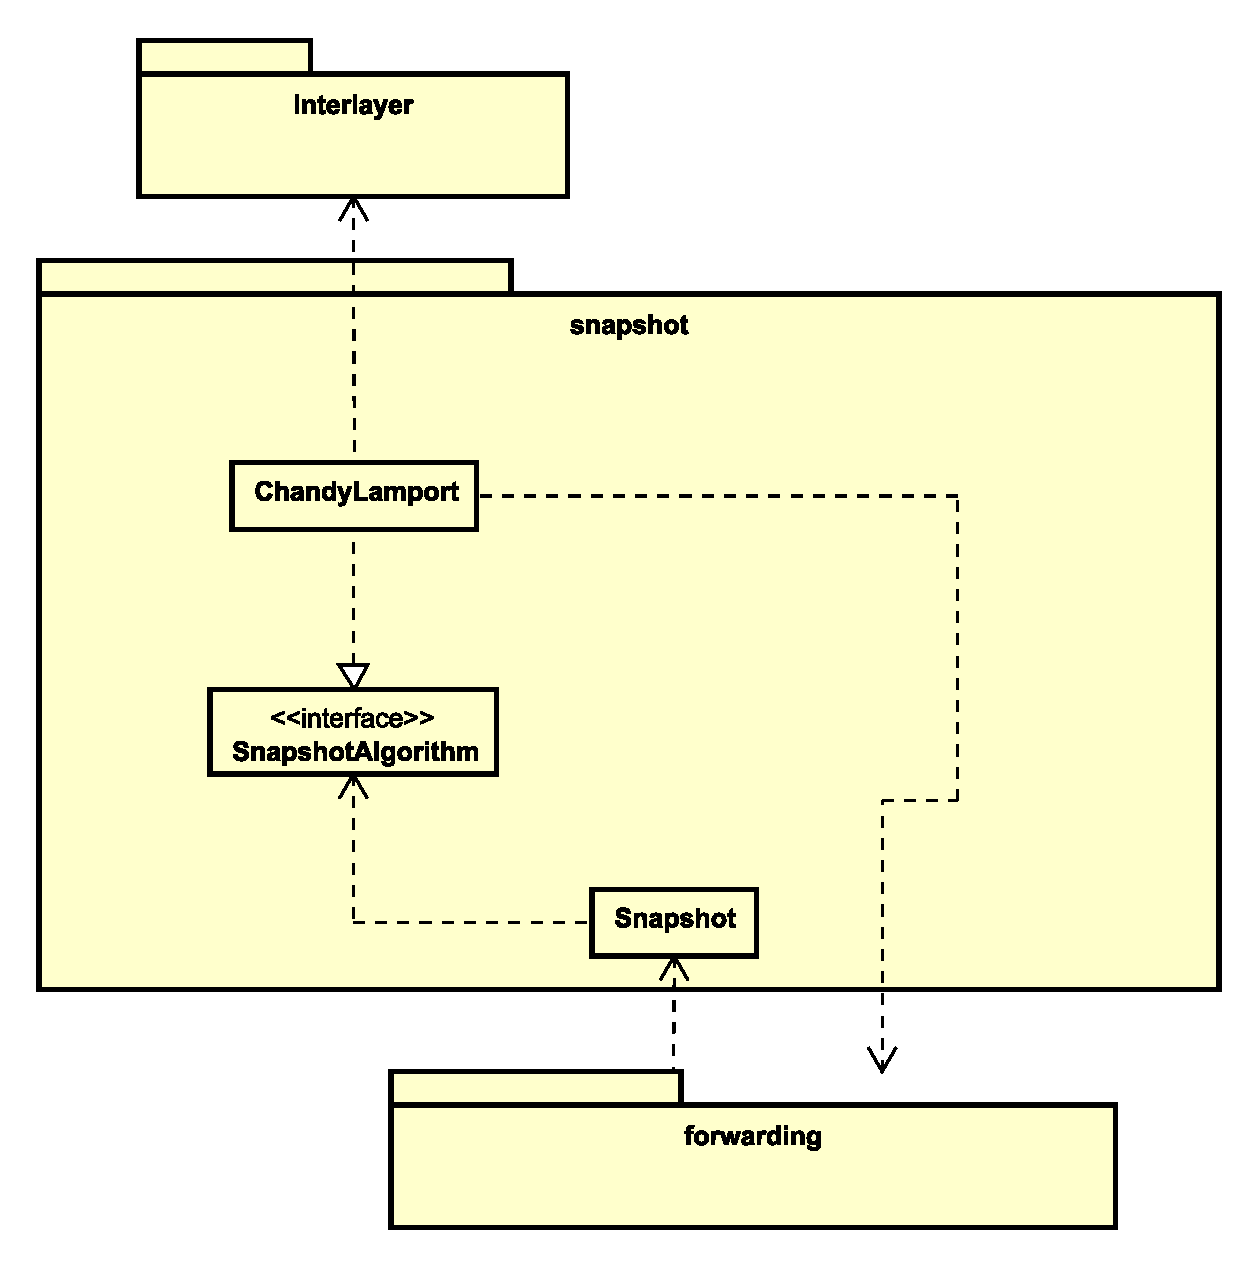
\includegraphics[width=\columnwidth]{images/solution/mw/snapshot.eps}
  \caption{Middleware's Snapshot service}
  \label{fig:mw-snapshot}
\end{figure}

% TODO: All class diagrams have to be added
\subsubsubsection{snapshot.Snapshot}
% TODO: Class diagram
\FloatBarrier
\begin{itemize}
  \item \textbf{Description} \\
    This module is the Fa\c cade of the Snapshot service. It is responsible
    to boot neatly and supervise all processes in Snapshot. Also, it has to
    handle snapshot requests that come from other nodes of the system.
  \item \textbf{Attributes}
  \item \textbf{Operations}
  \begin{itemize}
    \item \texttt{+ start()} \\
    Starts the Snapshot service.
    \item \texttt{+ handleMessage(message: String)} \\
    % TODO: check this out: Message will really be a String?
    Handles a snapshot start/termination request that comes from other nodes
    or receives snapshot information from the application layer.
  \end{itemize}
\end{itemize}

\subsubsubsection{snapshot.SnapshotAlgorithm}
% TODO: Class diagram
\FloatBarrier
\begin{itemize}
  \item \textbf{Description} \\
    Interface for processes that implement a certain kind of snapshot.
  \item \textbf{Attributes}
  \item \textbf{Operations}
  \begin{itemize}
    \item \texttt{+ take()} \\
    Starts to take a snapshot.
    \item \texttt{+ submitLocalSnapshot()} \\
    Stores a local snapshot.
    \item \texttt{+ submitRemoteSnapshot()} \\
    Stores a remote snapshot.
  \end{itemize}
\end{itemize}

\subsubsubsection{snapshot.ChandyLamport}
% TODO: Class diagram
\FloatBarrier
\begin{itemize}
  \item \textbf{Description} \\
    Module that implements the \texttt{snapshot.SnapshotAlgorithm}
    interface to take snapshots with the algorithm by Chandy and Lamport.
  \item \textbf{Attributes}
  \item \textbf{Operations}
  \begin{itemize}
    \item \texttt{+ take()} \\
    Starts to take a snapshot: that implies Forwarding module to notify
    other nodes of that and to hold messages until the snapshot is over; also
    that implies Interlayer to issue a snapshot request to the application
    layer.
    \item \texttt{+ submitLocalSnapshot()} \\
    Stores the snapshot of the node where the process is executing.
    \item \texttt{+ submitRemoteSnapshot()} \\
    Stores the snapshot of a remote node.
  \end{itemize}
\end{itemize}

\subsubsection{Coordination service}

This component is responsible of the coordinating middleware nodes by
providing mechanisms with which the system is able to operate cohesively.

We show in figure \ref{fig:mw-coordination} the architecture of this service
and then we will show in detail each module that composes this component.

%\begin{figure}[H]
%  \centering
%  \includegraphics[width=\columnwidth]{images/solution/mw/coordination.eps}
%  \caption{Middleware's Coordination service}
%  \label{fig:mw-coordination}
%\end{figure}
% TODO: Add diagram

% TODO: All class diagrams have to be added
\subsubsubsection{coordination.Coordination}
% TODO: Class diagram
\FloatBarrier
\begin{itemize}
  \item \textbf{Description} \\
    This module is the Fa\c cade of the Coordination service. It is responsible
    to boot neatly and supervise all processes in Coordination.
  \item \textbf{Attributes}
  \item \textbf{Operations}
  \begin{itemize}
    \item \texttt{+ start()} \\
    Starts the Coordination service.
    \item \texttt{+ handleMessage(message: String)} \\
    % TODO: check this out: Message will really be a String?
    Receives a message and delegates the proper handling of it to an internal
    module.
  \end{itemize}
\end{itemize}

\subsubsubsection{coordination.coordinationInfo}
% TODO: Class diagram
\FloatBarrier
\begin{itemize}
  \item \textbf{Description} \\
    Process that holds the current state of the coordination.
  \item \textbf{Attributes}
    \begin{itemize}
      \item \texttt{- state: Map<Atom,Any>} \\
    Information about coordination.
    \end{itemize}
  \item \textbf{Operations}
  \begin{itemize}
    \item \texttt{+ startLink()} \\
    Starts the process and initialize \texttt{state} as an empty map.
    \item \texttt{+ getInfo(key: Atom)} \\
    Returns the information contained in the state at the entry \texttt{key}.
    \item \texttt{+ setInfo(key: Atom, value: Any)} \\
    Modifies the state held by the process by setting the entry \texttt{key}
    to the value \texttt{value}.
  \end{itemize}
\end{itemize}

\subsubsubsection{coordination.election.Election}
% TODO: Class diagram
% TODO: Explode class in interface and implementation
\FloatBarrier
\begin{itemize}
  \item \textbf{Description} \\
    Process that is responsible to manage the election of a system coordinator.
  \item \textbf{Attributes}
    % TODO
  \item \textbf{Operations}
    % TODO
\end{itemize}

\subsubsubsection{coordination.time.HeartbeatMaker}
% TODO: Class diagram
\FloatBarrier
\begin{itemize}
  \item \textbf{Description} \\
    Process that has to produce an heartbeat (i.e., a signal that represents
    the logical clock ticking in the system) for all the nodes in the
    system.
  \item \textbf{Attributes}
  \item \textbf{Operations}
  \begin{itemize}
    \item \texttt{+ start()} \\
    Starts HeartbeatMaker process.
    \item \texttt{+ enable()} \\
    Makes HeartbeatMaker begin producing heartbeats.
    \item \texttt{+ disable()} \\
    Makes HeartbeatMaker stop producing heartbeats.
  \end{itemize}
\end{itemize}

\subsubsubsection{coordination.time.HeartbeatListener}
% TODO: Class diagram
\FloatBarrier
\begin{itemize}
  \item \textbf{Description} \\
    Process that listens to heartbeats. It is responsible to delivering them
    to the application layer.
  \item \textbf{Attributes}
  \item \textbf{Operations}
  \begin{itemize}
    \item \texttt{+ start()} \\
    Starts HeartbeatListener process.
    \item \texttt{+ beat()} \\
    Notifies the application layer of a new heartbeat.
  \end{itemize}
\end{itemize}

